% paper2_cvm.tex — paper 2（CVM 2027 投稿，匿名版）。目标：摘要 2026-10-23 / 全文 2026-10-26，AoE；<=14 页含参考文献。
% 数字纪律：正文测量数字带 "% gate2:" 工件键注释，只取自工件，禁手写/估算。
% 匿名：提交版不得含单位/致谢/项目号；前作栈统一以 `Prior RGB-D stack` 指称（真名不入正文与 biblio）。
% 结构校准 / 叙事锁定 / 禁语清单等内部记录见 papers/paper2/INTERNAL_tex_notes.md（不入投稿件）。

\documentclass[10pt,twocolumn,letterpaper]{article}

\usepackage{cvm}
\usepackage{newtxtext}
\usepackage{epsfig}
\usepackage{graphicx}
\graphicspath{{figs/}}
\usepackage{amsmath}
\usepackage{amssymb}
\usepackage{booktabs}   % 三线表（\toprule/\midrule/\bottomrule）

% Include other packages here, before hyperref.
\usepackage{cite}   % 多引用按数字升序（CVM 模板要求 numerical order）
\usepackage[pagebackref=true,breaklinks=true,letterpaper=true,colorlinks,bookmarks=false]{hyperref}

\newcommand{\keywords}[1]{{\bf \emph{Keywords: #1}}}

% \cvmfinalcopy % *** Uncomment this line for the camera-ready version

\def\cvmPaperID{****} % *** Enter the cvm Paper ID here
\def\httilde{\mbox{\tt\raisebox{-.5ex}{\symbol{126}}}}

% Pages are numbered in submission mode, and unnumbered in camera-ready
\ifcvmfinal\pagestyle{empty}\fi

% Draft-only marker for numbers pending gate-2 verification.
\newcommand{\gate}[1]{{#1}} % 所有 \gate{...} 内的数字：gate2 前须逐个对工件复核
% 版面压紧（2026-10-17）：全文 12 个 float 用 LaTeX 默认 \textfloatsep=20pt，累计浪费可观。
% 加 Niedermayr 行后 14 页硬顶顶破，按「压 float 高度而非削正文」的既有结论收紧此处。
\setlength{\textfloatsep}{16pt plus 2pt minus 2pt}
\setlength{\floatsep}{10pt plus 2pt minus 2pt}
\setlength{\intextsep}{10pt plus 2pt minus 2pt}
% 参考文献页（2026-10-22）：v8.18 正文增补后参考文献尾部溢出到第 15 页；只压文献列表行距，
% 不动正文可读性。\footnotesize + 收紧 \itemsep 是老手稿的常规做法。
\let\oldthebibliography\thebibliography
\renewcommand{\thebibliography}[1]{%
  \oldthebibliography{#1}\footnotesize
  \setlength{\itemsep}{0pt}\setlength{\parsep}{0pt}\setlength{\parskip}{0pt}}

\begin{document}

%%%%%%%%% TITLE
\title{A Dynamic-Scene Gaussian SLAM Map: Anatomy, Compression, and Offline Repair}

\maketitle
% \thispagestyle{empty}

%%%%%%%%% ABSTRACT
\begin{abstract}
    Dynamic-scene RGB-D SLAM systems built on 3D Gaussian splatting keep moving content
    out of the map, and the artifact they store and reload is that map, not the trajectory.
    Gaussian-map compression takes trained static or 4D models as input; the map a
    dynamic-scene SLAM system writes at run time has not been characterised as an input
    distribution. We study the map of one such system, a dense RGB-D splatting SLAM stack
    with an anti-dynamic mask.
    Opening the stored map shows 30\% of its bytes to be bookkeeping the rasteriser never
    reads. A plain codec, uniform per-map quantisation with entropy coding and no learned
    parameters, compresses the frozen map $6\times$ at ${\sim}0.01$\,dB of
    rendered PSNR loss and $15\times$ at an aggressive point, and compresses the repair
    operator's layered output to ${\sim}8\times$ near-lossless; a post-hoc learned
    compressor lands within 10\% of that point, buying little beyond the quantisation
    choice. Erasing dynamic content costs $17.9$--$22.2$\,dB in the erased regions; an
    offline repair operator restores $5.5$--$9.0$\,dB of it with no static-region damage
    beyond $\pm0.25$\,dB, at $11$--$30$\% of the producing run's wall-clock. A second
    dynamic GS-SLAM system also stores non-unit quaternions and a weaker heavy tail, but
    not the bookkeeping composition or the near-isotropic scale bulk; a held-out panel
    from the same two benchmarks (BONN, TUM) reproduces the codec's working points.
\end{abstract}

\keywords{dynamic scenes, 3D Gaussian splatting, SLAM, map compression, offline repair}

\begin{figure}[t]
\centering
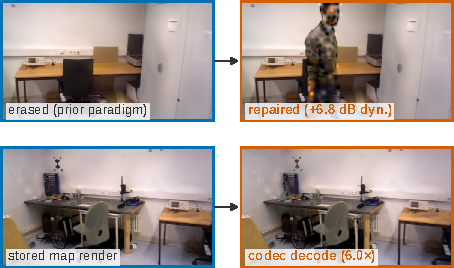
\includegraphics[width=\linewidth]{fig_teaser.pdf}
\caption{The anti-dynamic policy keeps online tracking robust, and it costs
\gate{17.9--22.2}\,dB in the erased regions (\S\ref{sec:dyncost}). Offline, on the
frozen map, the codec compresses \gate{6.0$\times$} at \gate{$\sim$0.01}\,dB loss,
and the repair operator restores the erased dynamic content (\gate{+6.8}\,dB
three-sequence mean: \emph{crowd2}, \emph{balloon2}, \emph{person\_tracking2}; static
regions untouched; \S\ref{sec:offline}).} % gate2: dyn_cost_5seq_2026-10-05.md (bad-region gain) + rd/l2_summary.json (6.0x) + dynport_offline_L1_{crowd2,balloon2,person_tracking2}_samepose.json (J1 medians, mean 6.82)
\label{fig:teaser}
\end{figure}

%%%%%%%%% BODY TEXT
\section{Introduction}
\label{sec:intro}

RGB-D SLAM built on 3D Gaussian splatting reconstructs a scene as a set of Gaussian
primitives that can be rendered in real time. In dynamic scenes the central difficulty
is deciding which pixels to trust. Moving people and objects violate the static-world assumption
that the map optimises against. The standard answer is an anti-dynamic
policy that keeps moving content out of the map, guided by a semantic mask.

Dynamic-scene SLAM is judged primarily by tracking error. But the artifact that is stored, shipped
and reloaded is not the trajectory; it is the map. This paper treats
the map of a dynamic-scene splatting SLAM system as a first-class object
(Fig.~\ref{fig:teaser}) and asks four
questions about it. What is actually inside such a map? How small can a plain offline
codec make it? What does the anti-dynamic policy cost on the map side? And can the
dynamic content it erases be put back offline?

The system whose maps we study is the authors' prior work~\cite{RoGSSLAM}, accepted for
publication at MMM 2027. It is a dense RGB-D splatting SLAM stack with an anti-dynamic mask,
used as-is in every experiment. \S\ref{sec:system} describes it in full. To place the map study in a
coordinate frame, we reproduce eleven published SLAM systems on the BONN dynamic
benchmark under one protocol and report them alongside the stack in
\S\ref{sec:system}; the reproduction shows the regime this paper targets, in which
most static methods diverge or degrade to tens of centimetres on dynamic sequences while
dynamic methods, including the stack used here, stay accurate.

Within that frame we make three map-side contributions. First, we open these maps and
find that 30\% of their raw bytes are constant bookkeeping the rasteriser never
reads, that a quaternion redundancy survives in the fields it does read and that a
near-isotropic scale bulk is available to a tighter coder, and that
the heavy tail is load-bearing (\S\ref{sec:accounting}). Second, we show that a
deliberately plain codec, uniform per-map quantisation ranges with entropy coding and no
learned parameters, reaches near-lossless \gate{$6\times$} compression at
\gate{$\sim$0.01}\,dB loss and \gate{$15\times$} at an aggressive working point, with the
gains traced to quantisation and verified on a held-out panel; the same scheme
compresses the repair operator's layered output to \gate{$\sim$8$\times$}
near-lossless by exploiting temporal smoothness and rotation redundancy
(\S\ref{sec:codec}). % gate2: rd/l2_summary.json (working points) + probe_4d_compress_2026-10-12.md (8x layered)
Third, we quantify the cost of the anti-dynamic policy. Erasing dynamic content costs
\gate{17.9--22.2}\,dB in the erased regions, most of it
recoverable by inserting the dynamic geometry back into the map
(\S\ref{sec:dyncost}); % gate2: dyn_cost_5seq_2026-10-05.md (bad-region PSNR gain)
and we show that an offline repair operator that moves
dynamic-content management out of the online loop restores the erased content with
\gate{5.5--9.0}\,dB of PSNR gain and no static-region damage beyond the
\gate{$\pm$0.25}\,dB band (\S\ref{sec:offline}). % gate2: manifest_offline_L1_L3.json (J1 range)

\begin{figure*}[t]
\centering
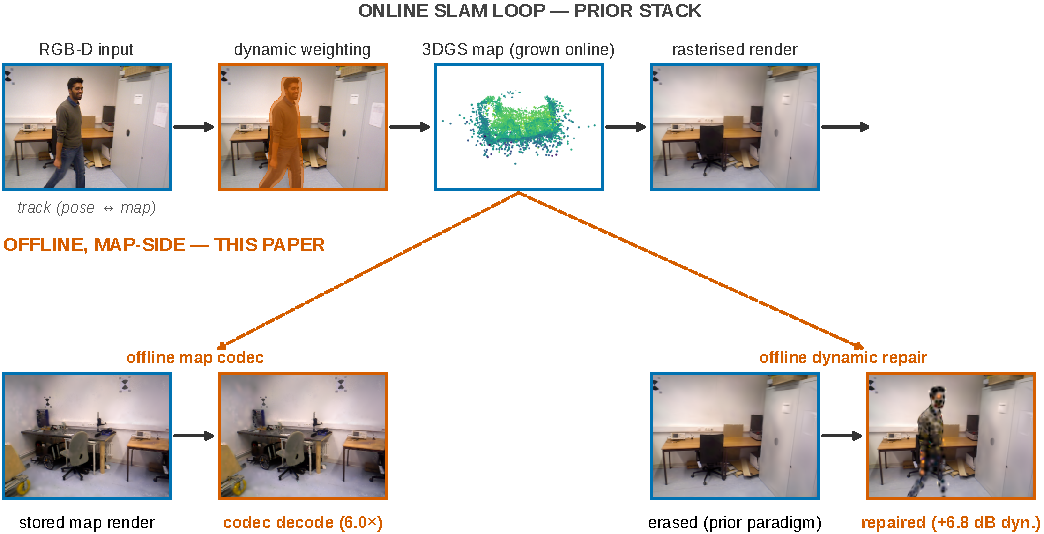
\includegraphics[width=0.68\linewidth]{fig1_pipeline.pdf}
\caption{System overview with real artifacts (\emph{crowd2} frame 621). Online (top, prior stack).
Each frame is tracked against the current Gaussian map, dynamic content
is masked rather than modelled, and the map grows under photometric and depth
supervision. Offline (bottom, this paper). A codec compresses the stored map
(\gate{6.0$\times$} over the 42 maps) and the repair operator restores erased dynamic
content at the same poses (\gate{+6.8}\,dB, three-sequence mean: \emph{crowd2}, \emph{balloon2}, \emph{person\_tracking2}).} % gate2: rd/l2_summary.json (6.0x) + dynport_offline_L1_{crowd2,balloon2,person_tracking2}_samepose.json (J1 medians, mean 6.82)
\label{fig:overview}
\end{figure*}

\section{Related Work}
\label{sec:related}

\paragraph{Optimisation-based splatting SLAM.}
3D Gaussian splatting \cite{Kerbl3DGS} has become the dominant map representation for
dense SLAM, replacing implicit fields with primitives that render in real time.
SplaTAM \cite{SplaTAM} introduced Gaussian maps for RGB-D SLAM with a silhouette-based
densification; MonoGS \cite{MonoGS} formulated tracking and mapping as a joint
photometric-geometric optimisation; Co-SLAM \cite{CoSLAM} is the corresponding
implicit-field baseline on the same benchmarks. Compactness of the representation has been studied
in this line. CGS-SLAM \cite{CGSSlam} and DiskChunGS \cite{DiskChunGS}
compress the Gaussian maps of static-scene SLAM systems, and importance-based pruning
was introduced by PWAS \cite{PWAS} and by the significance-guided pruning of
MGS-SLAM \cite{MGSSlam}. The codec here differs in the regime: the maps compressed come from a
dynamic-scene system with an anti-dynamic policy. The heavy tail, however, is not confined to
that regime (\S\ref{sec:accounting}), so it is carried rather than clipped.

\paragraph{Dynamic-scene handling.}
Dynamic content breaks the static-world assumption of splatting SLAM. The dominant answer is to
detect and erase. DynaSLAM \cite{DynaSLAM} inpaints dynamic regions in a classical pipeline,
NGD-SLAM \cite{NGDSLAM} masks them on an ORB-SLAM3 base and runs on CPU only, RoDyn-SLAM
\cite{RoDynSLAM} does the same with a neural implicit field, and among splatting systems DG-SLAM
\cite{DGSLAM}, WildGS-SLAM \cite{WildGS}, GGD-SLAM \cite{GGD}, RGD-SLAM \cite{RGDSLAM},
Dy3DGS-SLAM \cite{Dy3DGS} and BDGS-SLAM \cite{BDGSS} mask or down-weight dynamic
primitives during tracking and mapping. DGS-SLAM \cite{DGSSlam} is a separate,
contemporaneous system whose name differs from DG-SLAM by one letter; only DG-SLAM is
reproduced here. The opposite answer is to model the dynamics. DynaGSLAM \cite{DynaGSLAM} manages a
separate set of dynamic Gaussians with a
lifecycle, and the 4D line \cite{TC3DGS, MEGA} extends the representation over time.
The repair operator of \S\ref{sec:offline} adopts the DynaGSLAM management scheme but
moves it offline, applied to the finished map as a post-process instead of inside the
tracking loop.

\paragraph{Compact and compressible maps.}
Beyond SLAM-specific compression, 3DGS compression is an active area. HAC \cite{HAC}
and its successors learn entropy models over quantised attributes, Compact3D
\cite{Compact3D} and the compression survey \cite{CompressionSurvey} catalogue
attribute-wise schemes, SOG \cite{SOG} clips attribute ranges by percentiles, and
StitchGS \cite{StitchGS} prunes high-frequency SH parameters and quantises the rest.
TC3DGS \cite{TC3DGS} compresses dynamic scenes by
temporal grouping, and MEGA \cite{MEGA} by memory-efficient 4D representation. These
methods operate on trained static or 4D models; the maps of a dynamic-scene SLAM
system, with their constant bookkeeping fields and load-bearing heavy tail, are a
different input distribution, which is the gap \S\ref{sec:codec} addresses with a
parameter-free codec. % NOTE: tail_census inspected 14 maps (7 seq x 2 arms, seed 0); L2/L3 panels use 42/36.

\paragraph{Evaluation practice.}
Dynamic-scene SLAM is evaluated on the TUM \cite{TUMBenchmark} and Bonn
\cite{BonnDataset} benchmarks, and the dominant metric is ATE. Rendering quality is
reported as full-frame PSNR/SSIM/LPIPS following the protocol of MonoGS
\cite{MonoGS}. We additionally report metrics partitioned over the dynamic and static
regions throughout; the protocol is stated once in \S\ref{sec:system}. In contrast to the lines above, this work studies the map of a dynamic-scene
system as the object of interest. We open it, compress it with a plain codec, quantify what the
anti-dynamic policy erases, and repair the erased content
offline.

\section{System and Comparison}
\label{sec:system}

The system studied in this paper is a dense RGB-D splatting SLAM pipeline for dynamic
scenes. Each frame is tracked against the current Gaussian map; the map then grows under
photometric and depth supervision, while dynamic content is excluded from the map by a
semantic mask (Fig.~\ref{fig:overview}). The base design follows an optimisation-based
RGB-D splatting SLAM
\cite{MonoGS}, extended with four components: a Huber robust loss ($\delta=0.1$) on the
tracking residual, a per-pixel reliability signal, keyframe selection with a coverage gap
cap of five frames, and a deferred-commit lifecycle that prunes map primitives.
We report this stack as the \emph{Prior RGB-D stack}. It is the authors' prior work~\cite{RoGSSLAM},
accepted for publication at MMM 2027, used as-is in every experiment of this paper; its measurements are
placed here only as a coordinate frame, not as a result of this paper. % gate2: paper1_paper2_crosscheck_2026-10-05.md §2 (RobustTracking Huber delta=0.1; ReliabilitySignal; DynamicKeyframe gap_cap=5; DeferredCommit lifecycle deferred/prune)
The prior work ships two configurations, and every map-level number in this paper is
measured on both: the \emph{baseline arm} (the stack with the module switches off) and
the \emph{final arm} (the same stack with sliding-window pose correction and loop
closure switched on). Both arms share the mask pathway, the keyframe schedule and the
map schema, so a map from either arm is the same kind of object; we report them as
two arms of one system throughout, never as two systems. % gate2: configs/experiments/paper2_fulltable/{balloon_baseline,balloon_final}.yaml (SWBA.enabled + LoopClosure.enabled are the only switches)

To make that coordinate frame concrete, we reproduce eleven published SLAM systems on the
BONN dynamic benchmark \cite{BonnDataset}: the same machine, the same
evaluation harness, and Horn SE(3) alignment with the error in centimetres (mean and
standard deviation over three seeds; the protocol is stated once in the evaluation
paragraph below and the raw outputs are released at publication). Execution
conditions vary across systems: DynaSLAM and NGD-SLAM are classical keypoint
pipelines (DynaSLAM on an ORB-SLAM2 base, NGD-SLAM on an ORB-SLAM3 base, both
CPU-only), WildGS-SLAM is monocular, and seed reporting follows each system's
capability. These numbers establish the tracking regime this map study builds on,
not isolated map-architecture comparisons.
Table~\ref{tab:baseline} reports
the absolute trajectory
error (ATE) on the six BONN sequences shared between the reproduced systems and the prior stack
(\emph{balloon}, \emph{balloon2}, \emph{crowd}, \emph{crowd2}, \emph{person\_tracking},
\emph{person\_tracking2}); the reproduction covers eight sequences per system, and the two
extra ones available only to the baselines (\emph{mv\_no\_box}, \emph{mv\_no\_box2}) as well
as the \emph{crowd3} sequence available only to the prior stack are kept out of the table to avoid
mixing incomparable subsets.

% generated by scripts/02_analysis/paper2_baseline_table.py -- do not edit by hand
% provenance: resources/baselines/baselines_result/*/tracking_raw.csv
% 口径：Horn SE(3) / cm / ddof=1；公共 BONN 6 序列；格 = ATE mean±sd (cm)；-- = N/A
\begin{table*}[t]
\centering
\footnotesize
\setlength{\tabcolsep}{4pt}
\begin{tabular}{@{}llcccccc@{}}
\toprule
\emph{Method} & \emph{Family} & balloon & balloon2 & crowd & crowd2 & person\_tracking & person\_tracking2 \\
\midrule
\multicolumn{8}{@{}l}{\emph{Static methods}} \\
MonoGS & 3DGS & 39.32$\pm$1.01 & 22.05$\pm$1.55 & 86.47$\pm$18.34$^\mathrm{d}$ & 147.46$\pm$39.03$^\mathrm{d}$ & 44.83$\pm$9.06 & 43.85$\pm$8.55 \\
SplaTAM & 3DGS & 36.50$\pm$0.53 & 37.47$\pm$2.87 & 135.37$\pm$36.15$^\mathrm{d}$ & 493.22$\pm$470.66$^\mathrm{d}$ & 92.52$\pm$18.93$^\mathrm{d}$ & 132.72$\pm$9.37$^\mathrm{d}$ \\
Co-SLAM & implicit & 27.10$\pm$0.97 & 35.10$\pm$4.07 & 35866.32$\pm$38265.29$^\mathrm{d}$ & 24905.40$\pm$42817.31$^\mathrm{d}$ & 75.50$\pm$6.52 & 71.26$\pm$2.90 \\
ORB-SLAM3 & classical & 7.27$\pm$1.45 & 19.81$\pm$2.18 & 76.60$\pm$27.86$^\mathrm{d}$ & 111.41$\pm$14.75$^\mathrm{d}$ & 69.54$\pm$2.19 & 76.82$\pm$2.14 \\
\midrule
\multicolumn{8}{@{}l}{\emph{Dynamic methods}} \\
DG-SLAM & 3DGS & 3.66$\pm$0.02 & 3.83$\pm$0.08 & 5.76$\pm$0.15 & 6.39$\pm$0.50 & 4.25$\pm$0.06 & 6.12$\pm$0.13 \\
RGD-SLAM & 3DGS & 2.45$\pm$0.22 & 4.26$\pm$0.89 & 2.61$\pm$0.28 & 2.36$\pm$0.06 & 7.21$\pm$1.24 & 20.10$\pm$2.55 \\
WildGS-SLAM & 3DGS & 2.75$\pm$0.07 & 2.42$\pm$0.04 & 1.55$\pm$0.06 & 2.17$\pm$0.05 & 3.63$\pm$0.08 & 3.09$\pm$0.03 \\
DynaGSLAM & 3DGS & 8.36 & 9.36 & 23.82 & 13.73 & 8.94 & 13.69 \\
DynaSLAM & classical & 2.88$\pm$0.16 & 2.59$\pm$0.10 & 2.07$\pm$0.21 & 2.85$\pm$0.28$^\mathrm{d}$ & 4.53$\pm$1.81 & 8.82$\pm$1.18 \\
NGD-SLAM & classical & 2.82$\pm$0.07 & 2.46$\pm$0.08 & 1.85$\pm$0.16 & 2.22$\pm$0.07 & 4.97$\pm$0.44 & 6.63$\pm$0.43 \\
RoDyn-SLAM & implicit & 8.47$\pm$0.31 & 11.90$\pm$0.21 & 5.60$\pm$0.18 & 4.63$\pm$0.06 & 16.39$\pm$0.54 & 14.36$\pm$0.11 \\
\midrule
\textbf{Prior RGB-D stack} & \textbf{3DGS} & 3.25$\pm$0.07 & 5.48$\pm$0.27 & 2.23$\pm$0.10 & 2.26$\pm$0.32 & 11.31$\pm$0.70 & 10.40$\pm$0.28 \\
\bottomrule
\end{tabular}
\caption{Absolute trajectory error on the common BONN sequences (RMSE, cm, mean$\pm$sd over 3 seeds; all-frames, Horn SE(3) alignment). Family is the map representation. The first eleven rows are a single same-machine reproduction. DynaGSLAM delegates tracking to an external front-end (DynoSAM poses) and its three seeds are therefore deterministic, so it is reported without variance. The last row is the prior RGB-D stack, evaluated on the same machine and protocol in an independent batch; it is reported as background and is not a result of this paper. Execution conditions vary across systems: DynaSLAM and NGD-SLAM are classical keypoint pipelines (DynaSLAM on an ORB-SLAM2 base, NGD-SLAM on an ORB-SLAM3 base, both CPU-only), WildGS-SLAM is monocular, and seed reporting follows each system's capability; these numbers establish the tracking regime this map study builds on, not isolated map-architecture comparisons. Static methods degrade severely on the dynamic sequences, which is the regime this paper targets; they are shown to place the dynamic methods in context, not as straw men. $^\mathrm{d}$: tracking diverged (path length $>5\times$ GT or ATE $>100$\,cm) on initial run; re-run attempted under the same protocol with recommended settings. Values shown are from the re-run (diverged status retained where re-run also diverged). PSNR and FPS are in the text.}
\label{tab:baseline}
\end{table*}


The table makes the regime of this paper visible in one glance. Most static SLAM methods
reproduced under the same protocol fail outright on the dynamic sequences (Co-SLAM
\cite{CoSLAM} exceeds $10^4$\,cm of ATE on \emph{crowd} and \emph{crowd2}, marked as
diverged), and the rest of the static group degrades to tens or hundreds of centimetres
in most cells, whereas the dynamic methods mostly
stay in the single digits. The separation is not absolute, and we do not claim it as one.
ORB-SLAM3, a static method, holds \gate{7.27}$\pm$\gate{1.45}\,cm on \emph{balloon};
within the dynamic group,
RGD-SLAM reaches \gate{20.10}$\pm$\gate{2.55}\,cm on \emph{person\_tracking2} and
DynaGSLAM \gate{23.82}\,cm on \emph{crowd}, so both groups contain failures. % gate2: tables_paper2_preview.json (per-method ATE)
The prior
stack sits inside the dynamic group on its ATE
(\gate{3.25}$\pm$\gate{0.07}\,cm on \emph{balloon} up to \gate{11.31}$\pm$\gate{0.70}\,cm on
\emph{person\_tracking}; full per-sequence values in the table), % gate2: tables_paper2_preview.json (prior stack ATE)
which is the regime this paper targets. The maps studied in \S\ref{sec:accounting} and compressed in
\S\ref{sec:codec} come from a system that keeps dynamic content out of the map rather than
modelling it. The higher readings on \emph{person\_tracking} and
\emph{person\_tracking2} carry a global scale drift of \gate{$\sim$10--15\%},
which Sim(3) alignment removes with the same trajectory shape (bringing them to
\gate{$\sim$7.6}\,cm on both sequences). % gate2: tables_paper2_preview.json (sim3_ate_seeds)
We report the SE(3) numbers to stay on the same alignment as the reproduced systems, and
flag the scale drift only so that the reading is not mistaken for a shape error
(Fig.~\ref{fig:traj} shows a representative trajectory against ground truth).

Rendering quality and runtime, which the table does not report, follow the same split less cleanly.
Among the eight reproduced systems with a reported rendering
path, the three 3DGS dynamic methods reach a full-frame PSNR spanning \gate{6.97--25.14}\,dB
(DynaGSLAM \gate{6.97--22.14}\,dB, DG-SLAM \gate{19.75--23.67}\,dB, RGD-SLAM \gate{22.76--25.14}\,dB), while the other dynamic methods and the static methods fall in
\gate{14--20}\,dB with substantial overlap, for example WildGS-SLAM at \gate{15.6--18.7}\,dB and
Co-SLAM at \gate{14.2}$\pm$\gate{0.7}\,dB on \emph{crowd}; the prior stack renders at
\gate{21.8}\,dB on \emph{balloon}. % gate2: tables_paper2_preview.json (per-method PSNR)
Three of the reproduced systems (DynaSLAM
\cite{DynaSLAM}, NGD-SLAM \cite{NGDSLAM}, ORB-SLAM3 \cite{ORBSLAM3}) have no full-frame
rendering path under the reproduction protocol, so we report only the numbers that exist.
End-to-end frame rates range from \gate{0.2--2}\,FPS for the splatting and NeRF systems to
\gate{50--72}\,FPS for the feature-based NGD-SLAM and ORB-SLAM3; these are same-machine
measurements, not a throughput benchmark. % gate2: tables_paper2_preview.json (per-method FPS)
Table~\ref{tab:render} gives the prior stack's own full-image PSNR, SSIM and LPIPS per
sequence, and Table~\ref{tab:eff} its online efficiency; per-system values are in the
supplementary material (Tables~S3--S4).

% generated by scripts/02_analysis/paper2_tables.py -- do not edit by hand
% provenance: R33 same-batch (baseline/swbaonly/final/gate x 7 Bonn seqs x 3 seeds, all runs 2026-09-16, identical code)
% 口径提醒：本表数字全部来自 results/ 既有产物；入论文前须过 slam-critic 关卡②
\begin{table}
\begin{center}
\begin{tabular}{lccc}
\toprule
Sequence & PSNR (dB) & SSIM & LPIPS \\
\midrule
balloon & 21.80 & 0.852 & 0.273 \\
balloon2 & 18.72 & 0.808 & 0.316 \\
crowd & 19.92 & 0.829 & 0.274 \\
crowd2 & 19.50 & 0.823 & 0.297 \\
crowd3 & 17.04 & 0.778 & 0.345 \\
person\_tracking & 22.68 & 0.860 & 0.264 \\
person\_tracking2 & 22.72 & 0.861 & 0.249 \\
\bottomrule
\end{tabular}
\end{center}
\caption{Full-image rendering quality of the prior stack, offline rendering protocol sampled away from the keyframe grid. This is the full-image protocol; partitioned static-region numbers are in Table~\ref{tab:static}. LPIPS uses the standard AlexNet backbone; lower is better.}
\label{tab:render}
\end{table}

% generated by scripts/02_analysis/paper2_tables.py -- do not edit by hand
% provenance: R33 same-batch (baseline/swbaonly/final/gate x 7 Bonn seqs x 3 seeds, all runs 2026-09-16, identical code)
% 口径提醒：本表数字全部来自 results/ 既有产物；入论文前须过 slam-critic 关卡②
\begin{table}
\begin{center}
\footnotesize
\begin{tabular}{lccc}
\toprule
Sequence & FPS excl. & FPS conc. & excl./conc. \\
\midrule
balloon & 1.162 & 0.645 & 1.80$\times$ \\
crowd2 & 1.278 & 0.987 & 1.29$\times$ \\
person\_tracking & 1.128 & 0.879 & 1.28$\times$ \\
\emph{median} & 1.162 & 0.879 & 1.32$\times$ \\
\bottomrule
\end{tabular}
\end{center}
\caption{Online-phase efficiency of the prior stack (baseline arm). The two FPS columns are a single-variable comparison: the same code revision and the same three sequences, differing only in processes per GPU (one vs.\ two); the per-sequence ratio spans 1.28--1.80, so concurrency is real but modest, not the several-fold penalty a cross-revision comparison would suggest. FPS = frames / online time, one seed per sequence; the median row is over the three sequences.}
\label{tab:eff}
\end{table}


\begin{figure}[t]
\centering
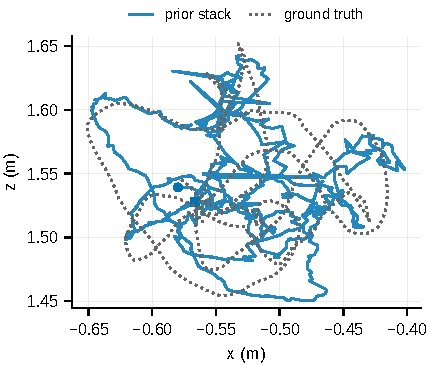
\includegraphics[width=0.90\columnwidth]{fig3_trajectory_crowd2.pdf}
\caption{Trajectory of the prior stack on \emph{crowd2} against ground truth (SE(3)
alignment, world frame). The stack tracks the dynamic sequence without divergence,
which is the regime the map study builds on.}
\label{fig:traj}
\end{figure}

Two limitations are intentional. First, the baselines and the prior stack were evaluated
in separate batches; they share the machine and protocol, and the caption marks this.
Second, we report the diverged rows as they are instead of clipping them. A static method that loses
track on a dynamic sequence is exactly the failure mode the anti-dynamic policy addresses.

\paragraph{Evaluation protocol.}
All measurements in this paper follow one protocol, stated here once and referenced from
each study. Tracking accuracy is reported as ATE RMSE in centimetres under Horn SE(3)
alignment, all frames, mean and standard deviation over three seeds (raw outputs
released at publication). Rendering metrics use the same offline
renderer for every arm and every sequence: a fixed evaluation frame set, the canonical
dynamic masks (single source of masks, rebuilt by one builder), and the full-frame plus
region-partitioned protocols described where each number is used. One reproduced system,
WildGS-SLAM, is monocular and receives RGB only; every other system receives RGB-D. Full-image PSNR
differs across tables only through the frame set. The codec tables (\S\ref{sec:codec}) render a
fixed evaluation set shared by all codec arms, while the system tables
(Table~\ref{tab:render}, Table~\ref{tab:static}) render a grid-away frame set of the
same maps, so absolute PSNR values are comparable within a table but not across the
two protocols. Numbers from different batches are never mixed in one table, and every
measurement in this paper is generated from logged artifacts by a script rather than
copied by hand.

\section{What a Dynamic-Scene Gaussian Map Is Made Of}
\label{sec:accounting}

Before designing anything that consumes a SLAM map, we open the map produced by the
prior stack on the dynamic sequences and ask what is actually stored in it. The stack is
the authors' prior work~\cite{RoGSSLAM}, used here as the primary study object; a
cross-system check on the anatomy only closes this section.
The representation is the standard 3D Gaussian one. Each primitive carries position,
opacity, scale, rotation and a colour term, stored on disk as 20 float32 values
(\gate{80}\,bytes per primitive at SH degree 0; \gate{14} of the fields, \gate{56}
bytes, are read by the rasteriser) % gate2: storage_census_2026-10-05.md §1
\cite{Kerbl3DGS}. The remaining \gate{6} fields (\gate{24}\,bytes, \gate{30\%} of the
raw bytes) are bookkeeping that the renderer never reads. They are a static probability, an
observation count, an unmapped score, and a surface normal. % gate2: storage_census_2026-10-05.md §1
The maps themselves are small. Across the seven Bonn sequences the baseline maps hold
\gate{3.2--7.1$\times 10^4$}
primitives, or \gate{2.6--5.7}\,MB on disk in the 20-field form. % gate2: storage_census_2026-10-05.md §1-2 (baseline column)
Three findings fall out
of opening the map this way.

\paragraph{Dead weight, already paid for by the entropy coder.}
The six bookkeeping fields are constant across every map we inspected. The static probability is
identically \gate{0.7}, the observation count and unmapped score are
identically \gate{0}, and the normal is identically zero % gate2: l1_readout_2026-10-04.md §5
(std~$\approx 0$, one unique value). They carry no information in these files. Two consequences matter
for what follows. First, this is why a naive \emph{byte}-level view of a SLAM map overstates its
content. 30\% of it is schema, not scene. Second, the redundancy is already gone after the first
compression pass. Entropy-coding the 20 float fields instead of the \gate{14} renderer fields costs
only \gate{1.04$\times$} in rate. % gate2: l1_readout_2026-10-04.md §5 (20$\rightarrow$14 fields)
The dead fields are therefore an accounting fact about these map files, not a
free compression gain.

\paragraph{Redundancy inside the fields the renderer does read.}
Two structural redundancies survive in the renderer-facing fields, and they differ in
how far this paper takes them.
The rotation is
stored as a raw quaternion that the rasteriser renormalises at render time; across the
maps we measured, \gate{88.8--94.7\%} of the quaternions deviate from unit norm by
more than 1\%. % gate2: anatomy_census.json (panel ours_dynamic, rot_dev_frac; 14 maps, range 0.8880--0.9475)
The codec therefore stores three components and recovers the fourth from the unit
constraint, which costs \gate{0.29}\,dB at matched compression ratio in the layered
codec of \S\ref{sec:codec} (Table~\ref{tab:4d-ablation}, row 2) and is used in the
map codec as well.
The scale is nearly isotropic for a large part of the map, but how large a part depends on
the scene. For \gate{78--92\%} of the primitives in the dynamic maps studied here the ratio
between the largest and smallest scale axis is below \gate{0.1} in log domain; on the two
clean static sequences the share falls to \gate{52--76\%}, and it is higher wherever people
are present (\gate{81--85\%} walking, \gate{89--91\%} seated). % gate2: anatomy_census.json (panels ours_dynamic / ours_heldout, iso_frac = aniso<0.1)
Storing the mean scale plus per-primitive deviations only for the anisotropic minority would
save \gate{23--48\%} of the scale group's bits depending on the working point (23--34\% at
8--10 bits, 34--48\% at 12 bits), measured on the dynamic maps.
% gate2: remeasured 2026-10-22 on the seven baseline seed-0 maps; scale-group zlib bytes, full vs mean+dev minority
Near-isotropy is thus a property of these maps under dynamic content, not of 3D
Gaussian maps in general: on DynaGSLAM's maps \gate{0.0--0.1\%} of primitives qualify
(median axis ratio \gate{2.30--2.56} in log domain, against \gate{0.003--0.008} in the
dynamic maps here).
The implementations differ in more than one respect (loss terms, densification, time
parameterisation) and we did not ablate them; a fixed isotropic regulariser in the mapping
loss is a candidate mechanism, not an established cause. % gate2: anatomy_census.json (panel dynagslam, 8 seq x 3 seeds)
The map codec studied here does \emph{not} implement this second form: the quantiser of
\S\ref{sec:codec} already absorbs part of the redundancy, and the measured end-to-end
gain is small (\gate{0.3--2.2\%} of the total bitstream). % gate2: checkpoint1_onepager_2026-10-04.md §5-bis (iso-scale 0.3-2.2%)
Fig.~\ref{fig:accounting} summarises the byte budget.

\begin{figure}[t]
\centering
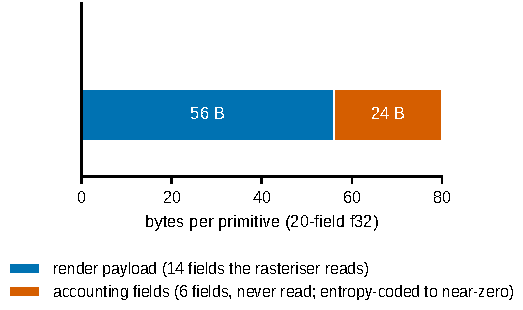
\includegraphics[width=0.89\columnwidth]{fig5_accounting.pdf}
\caption{Byte budget of one map primitive (20-field float32, SH degree 0). The rasteriser reads 14
of the 20 fields.}
\label{fig:accounting}
\end{figure}

\paragraph{The heavy tail is load-bearing.}
The scale distribution is heavy-tailed in a way that a generic compressor would not
expect. A robust range (0.1\% quantiles) is \gate{1.36--2.15$\times$} narrower than
the full range for the scale group and \gate{1.25--1.53$\times$} for positions across
the fourteen maps we inspected in detail (seven sequences $\times$ two arms, seed 0), % gate2: tail_census_2026-10-04.md §1 (seeds=[0], maps=14)
 and the tail is populated by genuinely large primitives. It is not a feature of dynamic
content: it persists on the clean static maps (\gate{1.40--1.79$\times$}, twelve maps) and
appears, weaker, in DynaGSLAM's maps (\gate{1.15--1.43$\times$}, twenty-four maps).
% gate2: anatomy_census.json (infl_scale, panels ours_heldout/dynagslam)
The maximum-axis scale of tail primitives
 exceeds that of the bulk by at least two log units, with dozens of the
largest primitives landing inside the tail % gate2: tail_census_2026-10-04.md §3
(top-100 $\cap$ tail). The tail is not disposable. Clipping the dynamic range of the
quantiser to the robust percentiles loses \gate{0.71}\,dB of full-frame PSNR
on \emph{crowd2} (and \gate{0.74}\,dB at the coarser working point), because the tail
holds primitives that render; carrying the tail through with an escape code keeps it
within noise of the full-range codec at a
\gate{5--15\%} rate premium. % gate2: verdict_l1b_robust_range_2026-10-04.md §2.2
 Range inflation is also not a reliable proxy for compressibility. The inflated groups are not the
 ones where robust ranges buy rendering quality. % gate2: qerr_probe_2026-10-04.md (ratio\_full) + verdict_l1b_robust_range_2026-10-04.md §5.2
Fig.~\ref{fig:tail} shows the tail and the per-sequence inflation.

\begin{figure}[t]
\centering
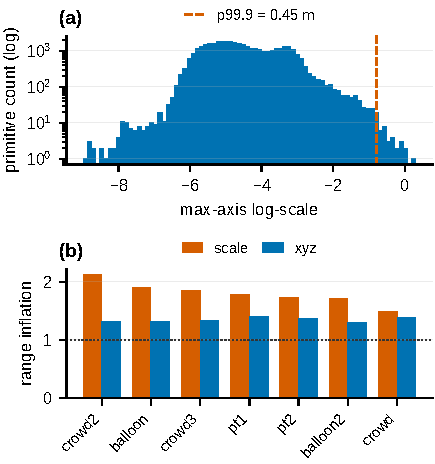
\includegraphics[width=\columnwidth]{fig4_tail.pdf}
\caption{Heavy tail of a dynamic-scene map (top, max-axis log-scale histogram of \emph{crowd2} with
the p99.9 line) and per-sequence range inflation (bottom, robust vs full range for scale and
position).}
\label{fig:tail}
\end{figure}

This map is therefore not what a generic compressor would assume. 30\% of its raw bytes are constant
schema, the rotation is safe to store in three components, the scale group has a
near-isotropic bulk that a tighter coder could exploit, and the
heavy tail must be carried. The second system keeps the non-unit rotation (\gate{96.5--98.6\%} of
its primitives, against \gate{88.8--94.7\%} here) and a weaker tail, but it stores only two
quaternion components, so the byte-level saving does not transfer; its schema is its own
(79 fields) and the near-isotropic bulk does not transfer.
Section~\ref{sec:codec} builds a deliberately plain codec on these findings, and takes the
rotation component of the first two.

\section{A Simple Baseline Codec for Gaussian Maps}
\label{sec:codec}

The anatomy of \S\ref{sec:accounting} suggests a compressor that any reader would write down first.
Quantise each attribute group to a fixed bit width, entropy-code the result,
and keep the heavy tail by choosing ranges that fit it. That is the codec we study, and
the point of this section is that such a deliberately plain codec already reaches
near-lossless $6\times$ on the frozen dynamic-scene maps, with the gains traced to
quantisation rather than to any learned component.

\paragraph{Design.}
Each primitive's attributes are grouped as position (xyz, three fields), colour
(f\_dc, three fields), opacity (one field), scale (three fields) and rotation. The
rotation group is stored as the three non-leading quaternion components after
normalisation, with the leading sign fixed non-negative and the fourth component
recovered from the unit constraint, so the group carries three fields rather than four.
Each group is quantised to a fixed bit width with a uniform range computed from that
map's own data, and the quantised stream is entropy-coded with zlib.
Writing $a$ for one attribute of one group, the codec stores
$q=\mathrm{round}\big((a-\ell)/(u-\ell)\cdot(2^{b}-1)\big)$ clipped to
$[0,2^{b}-1]$, where $b$ is the group's bit width and $\ell,u$ are that map's own
minimum and maximum for the group; decoding inverts the map. Both endpoints are carried
in the header, not fitted to any panel.
The bit widths are the only design choices and are the same three working
points for every map, quoted in the order
xyz/f\_dc/opacity/scale/rotation: near-lossless
\gate{16/8/8/8/8}, mid \gate{10/6/6/6/6}, aggressive \gate{8/4/4/4/4}. % gate2: rd/l2_summary.json (working points)
Only the per-map quantisation ranges are derived from each map's data, so nothing in
the codec is fitted to the held-out panel. The codec is parameter-free. No learned weights anywhere.
Decoding restores a standard PLY consumed by the same rasteriser as the source map.

\paragraph{Rate--distortion.}
We call a working point near-lossless when the full-image PSNR change stays within
\gate{$\pm$0.25}\,dB of the source, the same band used for the static-region
criterion in \S\ref{sec:offline}; the near-lossless point of Table~\ref{tab:rd}
lands far inside it.
Table~\ref{tab:rd} reports the rate--distortion behaviour on the frozen maps of the
seven Bonn sequences (baseline and final arms, three seeds; 42 maps) plus a held-out
panel of five TUM sequences and one Bonn sequence (36 maps) that never entered any
design choice. The near-lossless point compresses to \gate{5.96$\times$} at
\gate{$-0.01$}\,dB of full-image PSNR (full-image over the fixed codec evaluation
set, including masked dynamic regions, \S\ref{sec:system}); mid reaches
\gate{8.77$\times$} and aggressive \gate{15.11$\times$} at \gate{$-0.64$}\,dB.
% gate2: rd/l2_summary.json (global rows); lossless band: posthoc_baselines_2026-10-09.md
The lossless generic compressors bound the free ratio at \gate{1.37--1.62$\times$}
(Table~\ref{tab:rd}).
We also run a post-hoc learned compressor on the same frozen maps. SOG \cite{SOG} compresses
unsorted Gaussians without retraining. On these maps its unquantised mode reaches \gate{1.81$\times$}
at \gate{$0.00$}\,dB and its quantised mode
\gate{6.53$\times$} at \gate{$-0.02$}\,dB (per-configuration detail in supplementary Table~S6),
within 10\% of the parameter-free
codec's near-lossless point, and far below the \gate{19.9--39.5$\times$} it reports
on trained static scenes. % gate2: rd/learned_sog_L2.json; 19.9--39.5x = \cite{SOG}
What a learned codec buys here is thus almost entirely its quantisation choice.
Niedermayr's pipeline \cite{Compressed3DGS} accepts a frozen map only by re-fitting it. 5000
supervised iterations reach \gate{6.15$\times$} at \gate{$+0.77$}\,dB.
% gate2: rd/learned_nied_L{2,3}.json（L2 42 图均值 6.151x / Δ+0.767；Δ>0 = QAT 再拟合）
Methods that learn their entropy model jointly with the scene (HAC \cite{HAC},
Compact3D \cite{Compact3D}) cannot consume a frozen map without per-map retraining.

% generated by scripts/gs_compress/paper2_codec_tables.py -- do not edit by hand
% provenance: rd/{l2_summary.json, l2s_summary.json, L3_*, L2_*_baseline.json, posthoc_baselines.json, learned_sog_L*.json, learned_nied_L*.json}; D2-025 L1/L2/L3 + P0-1 + post-hoc generic + learned baselines
\begin{table*}
\begin{center}
\footnotesize
% 行距压紧：14 页硬顶由本 float 高度支配（2026-10-16 加 Niedermayr 行后实测 15 页 ⇒ 压回 14）
\renewcommand{\arraystretch}{0.87}
\setlength{\tabcolsep}{4pt}
\begin{tabular}{@{}lcccrccr@{}}
\toprule
Method & quant. & comp. & B/prim & full PSNR & $\Delta$ & static PSNR & held-out $\Delta$ \\
\midrule
\multicolumn{8}{@{}l}{\emph{Source and lossless generic compressors}} \\
\quad source (uncompressed, 20-field f32) & -- & 1.00$\times$ & 80 & 15.38 & $0.00$ & 21.95 & $0.00$ \\
\quad zlib (lossless) & -- & 1.47$\times$ & 54.3 & 15.38 & $0.00$ & 21.95 & $0.00$ \\
\quad zstd (lossless) & -- & 1.54$\times$ & 51.8 & 15.38 & $0.00$ & 21.95 & $0.00$ \\
\quad lzma (lossless) & -- & 1.62$\times$ & 49.3 & 15.38 & $0.00$ & 21.95 & $0.00$ \\
\quad blosc2 (shuffle+delta) (lossless) & -- & 1.37$\times$ & 58.2 & 15.38 & $0.00$ & 21.95 & $0.00$ \\
\midrule
\multicolumn{8}{@{}l}{\emph{Lossy baselines: generic (rate only) and post-hoc learned}} \\
\quad blosc2 TRUNC\_PREC=16 (lossy) & -- & 2.84$\times$ & 28.1 & -- & -- & -- & -- \\
\quad blosc2 TRUNC\_PREC=8 (lossy) & -- & 3.80$\times$ & 21.1 & -- & -- & -- & -- \\
\quad SOG (JXL, quantised) & -- & 6.53$\times$ & 12.2 & 15.36 & $-0.02$ & 21.82 & $-0.04$ \\
\quad Niedermayr c3dgs (QAT 5k) & -- & 6.15$\times$ & 13.0 & 16.15 & $+0.77$ & 20.94 & $-0.01$ \\
\midrule
\multicolumn{8}{@{}l}{\emph{This paper: uniform quantisation + zlib codec (lossy)}} \\
\quad \textbf{near-lossless} & 16/8/8/8/8 & 5.96$\times$ & 13.4 & 15.37 & $-0.01$ & 21.79 & $-0.00$ \\
\quad \textbf{mid} & 10/6/6/6/6 & 8.77$\times$ & 9.1 & 15.32 & $-0.06$ & 21.64 & $-0.21$ \\
\quad \textbf{aggressive} & 8/4/4/4/4 & 15.11$\times$ & 5.3 & 14.74 & $-0.64$ & 19.21 & $-1.77$ \\
\midrule
\multicolumn{8}{@{}l}{\emph{Ablation: + voxel merge (not an operating point)}} \\
\quad near-lossless + voxel merge & 16/8/8/8/8 & 7.81$\times$ & 10.2 & 15.30 & $-0.08$ & -- & -- \\
\quad mid + voxel merge & 10/6/6/6/6 & 11.26$\times$ & 7.1 & 15.25 & $-0.13$ & -- & -- \\
\quad aggressive + voxel merge & 8/4/4/4/4 & 19.00$\times$ & 4.2 & 14.72 & $-0.66$ & -- & -- \\
\bottomrule
\end{tabular}
\end{center}
\caption{Rate--distortion on the frozen dynamic-scene maps (seven Bonn sequences, baseline and final arms, three seeds) and an unseen held-out panel (five TUM sequences, one Bonn). Compression ratio is the mean over per-map ratios in each group; compression is the source 20-field f32 map size over the stored bitstream; B/prim is bytes per primitive; PSNR is rendered full-image (static = static region); $\Delta$ is the change from the source (negative = loss), held-out $\Delta$ on the held-out panel. Lossless compressors render identically to the source, bounding only the free ratio ($\approx1.4$--$1.6\times$); the gain above them is from quantisation, not entropy coding. The codec is lossy and parameter-free. The blosc2 rows are rate-only (rendered quality not measured). SOG shares the denominator and instrument, its bookkeeping fields carried losslessly (\S\ref{sec:codec}). The Niedermayr row is refit, not post-hoc; its reference implementation seeds nothing, so per-map values are not reproducible beyond $\approx$0.1\,dB (\S\ref{sec:codec}). Voxel-merge rows are an ablation, not operating points (+26--31\% ratio at 0.02--0.07\,dB mean loss).}
\label{tab:rd}
\end{table*}

Fig.~\ref{fig:rd} shows the corresponding rate--distortion curves per sequence.

\begin{figure*}[t]
\centering
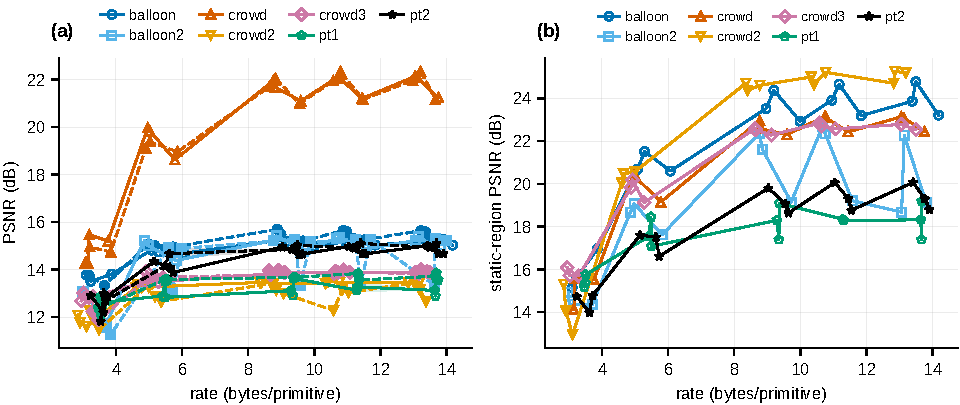
\includegraphics[width=0.82\linewidth]{fig_rd_curves.pdf}
\caption{Rate--distortion curves on the seven Bonn sequences (three-seed mean,
shaded band = interquartile range in panel (a) only). Left, full-image PSNR; right, static-region PSNR.
Solid = baseline arm, dashed = final arm.}
\label{fig:rd}
\end{figure*}

\paragraph{Voxel merging, and where it breaks.}
Merging primitives closer than \gate{2\,cm} in a voxel grid removes \gate{20\%} of the
primitives, which is why it appears as an ablation row rather than an operating point. % gate2: verdict_struct_codec_2026-10-05.md (L2S)
 The loss concentrates on the most crowded sequence, where the heavy tail of
\S\ref{sec:accounting} carries the most weight and the anti-dynamic policy leaves the most erased
content. Crowded dynamic scenes are precisely where primitives cannot be
dropped, whether by merging or by pruning.

\paragraph{Alternatives we tried, briefly.}
Several further allocation and encoding schemes (region- or visibility-aware bit
allocation, importance weighting, water-filling, trajectory-based pruning, Morton
delta coding, isotropic-scale collapse) were implemented at matched rate and none
improved the rate--distortion frontier. % gate2: l1_readout_2026-10-04.md §6.1-6.4
The closest is voxel merging, above. The redundancies of \S\ref{sec:accounting} are
already partly absorbed by the entropy coder, and the heavy tail rules out range-based
shortcuts.

\paragraph{Generalisation.}
The held-out panel (five TUM sequences: \emph{freiburg1\_desk2}, \emph{freiburg1\_room},
\emph{freiburg3\_long\_office\_household}, \emph{freiburg3\_sitting\_rpy}, and
\emph{freiburg3\_walking\_rpy}; plus one Bonn sequence, \emph{moving\_obstructing\_box},
never touched by any design choice) reproduces the working points: \gate{5.96$\times$} at near-lossless,
independently computed on the panel's 36 maps (per-map ratios span
\gate{5.72--6.12}; that the mean matches the frozen-map ratio of the same name is a
numerical coincidence, the panels being disjoint), with a full-image PSNR of
\gate{15.90}\,dB against the source's own \gate{15.90}\,dB,
and \gate{14.13}\,dB at aggressive. % gate2: rd/l3_generalization_2026-10-04.md (36 maps, global rows)
 The bit widths and the range procedure were fixed before the panel was rendered, so this
is an out-of-sample check, not a re-fit. The panel includes one dynamic TUM sequence
(\emph{freiburg3\_walking\_rpy}, a person walking in view); with a dynamic-region mask
generated by the same pipeline as the Bonn maps, the near-lossless point loses at most
\gate{0.008}\,dB of PSNR in the dynamic region across six runs (two arms, three seeds),
matching the static sequences. % gate2: rd/L3p_f3_wk_rpy_*_rd_table.json (dynamic-region ΔPSNR, 2026-10-13)
Split by scene class the working points barely move: \gate{5.92$\times$}/\gate{8.73$\times$}/\gate{14.84$\times$}
on the two clean static sequences against \gate{5.94$\times$}/\gate{8.60$\times$}/\gate{14.46$\times$} on the dynamic two.
% gate2: rd/L3_*_rd_table.json (ratio_full, clean static = f1_desk2+f3_office, dynamic = f3_wk_rpy+mob_box)

\paragraph{Cost.}
Encoding is a single-threaded CPU pass, taking \gate{0.7}\,$\mu$s per primitive at the
near-lossless point and \gate{7.4}\,$\mu$s at aggressive, with decoding at
\gate{0.13--0.15}\,$\mu$s per primitive across all points. % gate2: codec_timing_2026-10-05.md
The coarse working points cost \emph{more} to encode, not less: the quantiser itself is
indexing-bound and takes the same time at every bit width, while the deflate pass runs
longer on the lower-entropy stream. A map of tens of thousands of primitives encodes in
tens to hundreds of milliseconds. The per-map quantisation ranges are a few dozen bytes
of side information carried with the bitstream. The codec is offline by construction, so
this cost never enters the online loop.

\paragraph{Compressing the repaired layers.}
The same scheme extends to the repair operator's output of \S\ref{sec:offline},
which is a time-ordered sequence of per-frame dynamic layers. Two findings of \S\ref{sec:accounting}
carry over directly. The dynamic layers also carry a large share of suppressed primitives, whose
opacity the offline mask pruning of \S\ref{sec:offline} sets so low that they are invisible, and the
same rotation redundancy is present. Three further mechanisms help in the temporal
dimension. Primitives that persist across keyframes move smoothly (median per-step
displacement \gate{0.61}\,cm), so a constant-velocity predictor leaves a near-zero
residual that quantises almost losslessly. % gate2: probe_4d_compress_2026-10-12.md (trajectory smoothness)
Rotation is stored in three components
with the unit constraint, and per-attribute bit widths give more bits to positions
and fewer to opacity and rotation. The resulting codec reaches near-lossless
\gate{$\sim$8$\times$} compression of the layer sequence (\gate{8.1$\times$} on
\emph{crowd2}; \gate{7.9--9.3$\times$} across four sequences), with the dynamic-region
gain of \S\ref{sec:offline} largely preserved (J1 kept at \gate{84--96\%} of its
uncompressed value across the four sequences, per sequence in
Fig.~\ref{fig:rd-4d-gen}). % gate2: probe_4d_compress_2026-10-12.md (v3 working points + generalization)
Fig.~\ref{fig:rd-4d} shows the rate--distortion curve.
A higher-fidelity 12-bit working point compresses the same layers to
\gate{3.9--4.7$\times$} while keeping J1 at \gate{85--97\%} of its uncompressed
value, passing the same criteria on all four sequences. % gate2: probe_4d_compress_2026-10-12.md (12-bit generalization, 2026-10-13)

\paragraph{What each mechanism buys.}
On \emph{crowd2}, where the ablation is measured, the four mechanisms play different
roles. Suppressed-primitive exclusion is the largest lever. Without it the ratio drops from
\gate{8.12$\times$} to \gate{6.20$\times$} on \emph{crowd2}, because
the invisible primitives would otherwise dominate the quantisation range. % gate2: probe_4d_compress_2026-10-12.md (ablation, exclusion)
The
three-component rotation saves a smaller but consistent \gate{0.5$\times$}
(\gate{7.66$\times$} without it), at a precision cost of 0.29\,dB (J1 \gate{7.63}
vs \gate{7.92}\,dB, Table~\ref{tab:4d-ablation}). % gate2: probe_4d_compress_2026-10-12.md (ablation, rot3)
The constant-velocity predictor does not save bytes
at all (removing it raises the ratio to \gate{8.33$\times$}); its role is precision,
keeping J1 at \gate{7.63} instead of \gate{7.57}\,dB at the same bit budget. The
per-attribute bit widths allocate the budget where it matters: positions keep the
full width, opacity and rotation are quantised harder. % gate2: probe_4d_compress_2026-10-12.md (ablation table)
Table~\ref{tab:4d-ablation} summarises the ablation.

% generated by session 2026-10-12 (probe_4d_compress_2026-10-12.md ablation table)
% 口径：crowd2_R1 178 快照；判据机 samepose；修复后真实数字（链式赋值 bug 修复后）
\begin{table}[t]
\centering
\footnotesize
\setlength{\tabcolsep}{4pt}
\begin{tabular}{lcc}
\toprule
\emph{Configuration} & \emph{Ratio} & \emph{J1 (dB)} \\
\midrule
Full \gate{10/6/4/6/6} & \textbf{8.12$\times$} & 7.63 \\
w/o prediction & 8.33$\times$ & 7.57 \\
w/o rot3 & 7.66$\times$ & 7.92 \\
w/o suppression & 6.20$\times$ & 7.57 \\
\midrule
Uncompressed & 1.0$\times$ & 7.95 \\
\bottomrule
\end{tabular}
\caption{Ablation of the 4D layer codec on \emph{crowd2}. Removing the
suppressed-primitive exclusion costs the most ratio; removing the rotation
three-component form costs a smaller but consistent amount; removing the
constant-velocity predictor saves no bytes (the ratio rises) and only costs a
little precision. All variants keep the static region within criterion
(J3 $\in \pm 0.25$\,dB). J1 = dynamic-region PSNR gain vs the erased baseline.}
\label{tab:4d-ablation}
\end{table}


\begin{figure}[t]
\centering
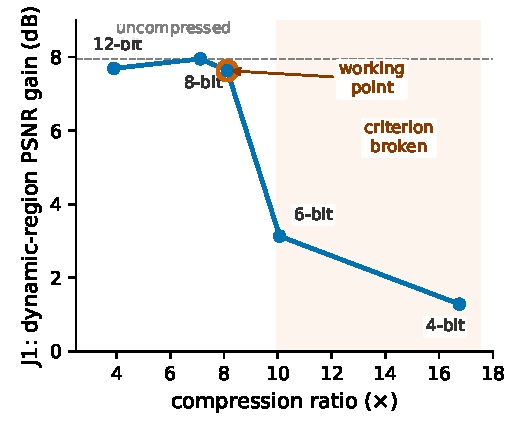
\includegraphics[width=0.89\columnwidth]{fig7_4d_rd.pdf}
\caption{Rate--distortion of the 4D layer codec on \emph{crowd2}. Dynamic-region PSNR gain (J1)
against compression ratio at increasing bit widths. Low bit widths
break the static-region criterion (shaded); the per-attribute working point
\gate{10/6/4/6/6} sits near the uncompressed gain at \gate{8.1$\times$}.} % gate2: probe_4d_compress_2026-10-12.md (working point 8.1x)
\label{fig:rd-4d}
\end{figure}

\begin{figure}[t]
\centering
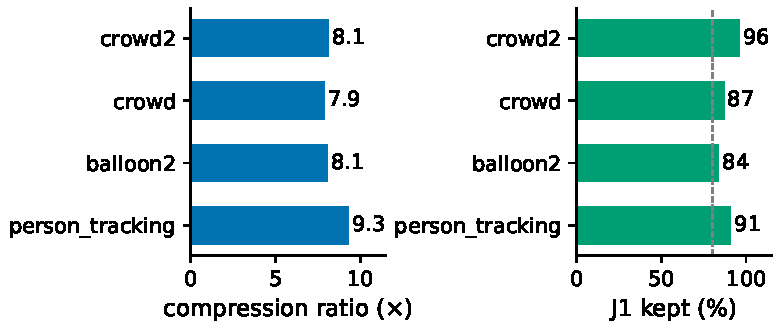
\includegraphics[width=0.89\columnwidth]{fig9_4d_gen.pdf}
\caption{The 4D layer codec across four sequences at the \gate{10/6/4/6/6} working point.
Compression ratio (left) and the dynamic-region gain J1 kept after
compression (right, percentage of the uncompressed value). The ratio is stable
across sequences and the gain stays above 80\%.} % gate2: probe_4d_compress_2026-10-12.md (generalization, 4 seq)
\label{fig:rd-4d-gen}
\end{figure}

Two boundaries are worth stating. The codec reads the single merged PLY that the
system saves, and the same quantisation applies to the layered output of the repair
operator as described above. The absolute map sizes here are a few megabytes, so the
honest unit of comparison is the ratio and bytes per primitive, not a headline
megabyte number.

\section{The Cost of the Anti-Dynamic Policy}
\label{sec:dyncost}

The comparison of \S\ref{sec:system} establishes why dynamic scenes need an anti-dynamic policy at
all. Static methods lose track outright. The policy itself, however, is not
free. This section quantifies what erasing dynamic content costs on the map side, using
the same frozen maps and the same offline renderer as \S\ref{sec:codec}, with the
dynamic regions defined by the canonical masks and the erased content measured against a
preserving counterfactual on the same frames.

\paragraph{Erasing dynamic content is expensive exactly where it matters.}
On five of the seven Bonn sequences (ten maps, excluding \emph{balloon} and \emph{person\_tracking2}),
re-inserting the dynamic content that the
anti-dynamic policy erased (under ground-truth depth, as the ground-truth-depth oracle) improves the PSNR inside the dynamic regions by
\gate{+17.9} to \gate{+22.2}\,dB and cuts the depth error there to \gate{15--27\%} of
its erased value, in every one of the ten maps (\gate{16--27\%} on the baseline arm
and \gate{15--24\%} on the final arm, Table~\ref{tab:dyncost-seq}; per-map values in supplementary
Table~S7). % gate2: dyn_cost_5seq_2026-10-05.md (bad-region PSNR gain and dl1 ratio)
 The gain is not an artifact of easy regions. It concentrates in the mask interior,
where the erased map renders a static background over pixels the dynamic object should
occupy (Fig.~\ref{fig:render} and Fig.~\ref{fig:render-pt}, two sequence types). Full-frame
PSNR improves by \gate{+5.4} to
\gate{+12.0}\,dB on the same runs. The cost scales with crowding. The three crowd sequences show the
largest gains (\gate{+21} to \gate{+22}\,dB), the single-object and single-person
sequences the smallest (\gate{+17.9} to \gate{+19.5}\,dB), % gate2: dyn_cost_5seq_2026-10-05.md (per-sequence rows)
and Fig.~\ref{fig:dyncost-seq} shows the per-sequence spread.

\begin{figure}[t]
\centering
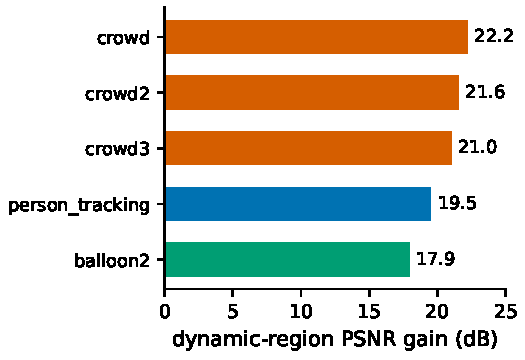
\includegraphics[width=0.90\columnwidth]{fig8_dyn_cost.pdf}
\caption{The erase cost is highest where the scene is most crowded. Dynamic-region
PSNR gain when the erased content is re-inserted, per sequence (baseline arm). The
three crowd sequences lose the most (21--22\,dB), the single-object scene the least.}
\label{fig:dyncost-seq}
\end{figure}

\begin{figure*}[t]
\centering
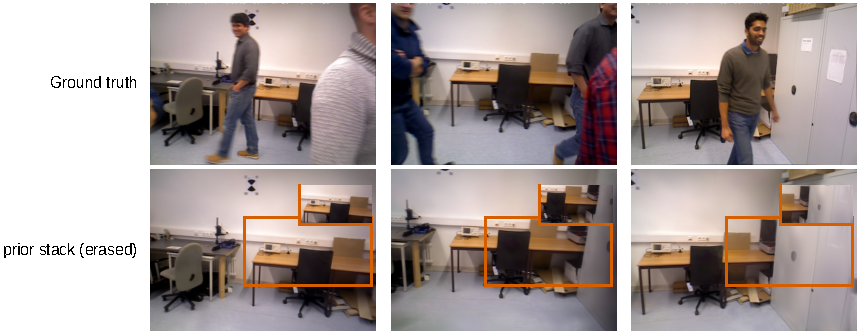
\includegraphics[width=0.58\linewidth]{fig2_render_crowd2.pdf}
\caption{Erase policy at its most visible. Top, ground truth. Bottom, the map with
dynamic content erased (prior stack). The vacated region left by the passing person is
a static-background hole; the inset shows where the dynamic object should be.}
\label{fig:render}
\end{figure*}

\begin{figure*}[t]
\centering
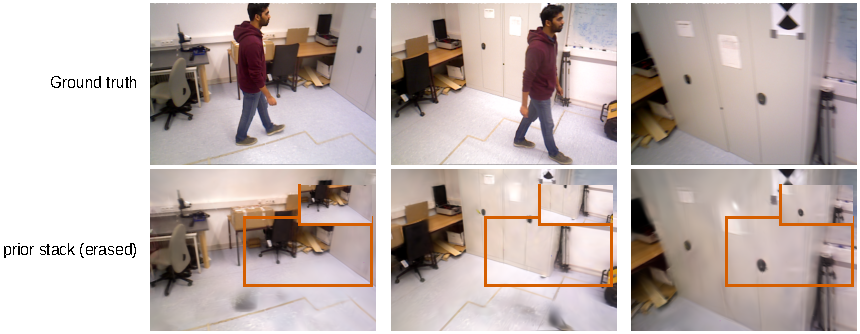
\includegraphics[width=0.58\linewidth]{fig2b_render_person_tracking.pdf}
\caption{The same effect on a second sequence (\emph{person\_tracking}), three frames.
Top, ground truth; bottom, the map with dynamic content erased. The erased map renders
the static background over the region the moving person occupies, the same failure mode
across sequence types; the orange inset marks where the person was.}
\label{fig:render-pt}
\end{figure*}

Table~\ref{tab:dyncost-seq} gives the per-sequence cost in full.

% generated by session 2026-10-12 (dyn_cost_5seq_2026-10-05.json, baseline arm)
% 口径：canonical 掩码分区；bad = M_bad（真损坏子集）；5 序列各 2 图（baseline+final）取 baseline
\begin{table}[t]
\centering
\footnotesize
\setlength{\tabcolsep}{4pt}
\begin{tabular}{lcccc}
\toprule
\emph{Sequence} & \emph{Dyn. gain} & \emph{Dyn. dL1} & \emph{Full} & \emph{Static} \\
 & \emph{(dB)} & \emph{ratio} & \emph{(dB)} & \emph{(dB)} \\
\midrule
crowd & 22.2 & 0.19 & +12.0 & +0.29 \\
crowd2 & 21.6 & 0.18 & +10.6 & +0.04 \\
crowd3 & 21.0 & 0.19 & +10.4 & +0.39 \\
person\_tracking & 19.5 & 0.27 & +8.7 & +0.28 \\
balloon2 & 17.9 & 0.16 & +5.4 & +0.33 \\
\bottomrule
\end{tabular}
\caption{The cost of the anti-dynamic policy per sequence (baseline arm). Columns:
dynamic-region PSNR gain when the erased content is re-inserted; the depth-error
ratio in the same region (lower is better); the full-frame gain; and the change in
the static region. The crowd sequences lose the most in the dynamic regions and
recover the most on re-insertion; no sequence damages the static region (all static
changes are positive, \gate{+0.04} to \gate{+0.39}\,dB).} % gate2: dyn_cost_5seq_2026-10-05.md (static Δ column, baseline)
\label{tab:dyncost-seq}
\end{table}


\paragraph{Most of the cost is recovered by geometry, not by motion modelling.}
A counterfactual decomposition on the same frames asks how much of the erased content
can be recovered by inserting the dynamic geometry alone, without modelling motion.
The decomposition uses two probes, and we name them separately because their residuals
are not the same quantity.
The \emph{ground-truth-depth oracle} inserts geometry unprojected from ground-truth depth at the
density the map saw during mapping. It is an oracle ceiling: it measures what the erased
content is worth, not what any system achieves.
The \emph{sensor-depth probe} inserts instead the geometry unprojected from the sensor
depth the mapping stage actually saw, with no motion model, and is the realistic
counterpart of that ceiling. Both insertions render
with the map's own Gaussian parameters and lighting, so the ceiling bounds the
recoverable content rather than reproducing the original frames.
Within that ceiling, the sensor-depth probe recovers \gate{0.80--0.93} of
the
oracle-recoverable depth error, leaving the dynamic-region depth error at
\gate{0.22--0.38} of its erased value, while freezing the inserted content at its
first observation retains only \gate{0.10--0.39}. % gate2: dyn_cost_decomp_2026-10-05.md (retention P2c vs P4, canonical 5seq; P2c/P1 residual = 1 - retention(P2c)*(1 - bad_dl1_ratio) = 1 - [0.80,0.93]*(1-[0.16,0.27]) = [0.22,0.38])
 The dominant term of the anti-dynamic cost is therefore missing geometry, not missing motion. The
 erase policy pays for content it never inserts, and most of that content
can in principle be put back by a static insertion. The insertion itself is cheap in map terms. It
adds \gate{6--29\%} additional primitives (median \gate{22\%}). % gate2: dyn_cost_decomp_2026-10-05.md (cost column)
Section~\ref{sec:offline} then asks how much of this recoverable gain a realisable operator
achieves under sensor depth and static preservation, and what mechanism pays for the
difference.

\paragraph{The static side is not the price.}
The same decomposition confirms that the erase policy does not buy its dynamic-region savings by
damaging the static map. Across the ten maps of both arms, nine change the static-region PSNR by
\gate{+0.04} to \gate{+0.39}\,dB, a slight improvement, and the tenth by \gate{$-0.03$}\,dB, so no
map degrades beyond the \gate{0.25}\,dB band; the
baseline arm alone is positive on all five sequences (Table~\ref{tab:dyncost-seq}). % gate2: dyn_cost_5seq_2026-10-05.md (static Δ column, 10 maps)
 Table~\ref{tab:static} reports the partitioned static metrics per sequence, including
the ghost excess left where dynamic content was removed.

% generated by scripts/02_analysis/paper2_tables.py -- do not edit by hand
% provenance: R33 same-batch (baseline/swbaonly/final/gate x 7 Bonn seqs x 3 seeds, all runs 2026-09-16, identical code)
% 口径提醒：本表数字全部来自 results/ 既有产物；入论文前须过 slam-critic 关卡②
\begin{table*}
\begin{center}
\footnotesize\renewcommand{\arraystretch}{0.94}
\begin{tabular}{lcccl}
\toprule
Sequence & static PSNR & static SSIM & ghost excess (cm) & mask source \\
\midrule
balloon & 27.68 & 0.911 & $2.97$ & dynamic\_mask \\
balloon2 & 26.28 & 0.902 & $-10.85$ & dynamic\_mask \\
crowd & 27.61 & 0.923 & $1.45$ & dynamic\_mask \\
crowd2 & 27.45 & 0.922 & $4.43$ & dynamic\_mask \\
crowd3 & 24.79 & 0.919 & $4.54$ & dynamic\_mask \\
person\_tracking & 27.31 & 0.901 & $3.96$ & dynamic\_mask \\
person\_tracking2 & 27.74 & 0.893 & $2.21$ & dynamic\_mask \\
\bottomrule
\end{tabular}
\end{center}
\caption{Partitioned metrics on the static support of the prior stack ($M_{\mathrm{static}} = $ valid GT depth $\wedge$ $\neg$dynamic, frozen method-independent masks). All rows use the same canonical static protocol: offline 6-frame rendering with the \texttt{dynamic\_mask} canonical masks (single-source masks, 84 runs). Ghost excess is the depth-L1 contrast between newly vacated regions and the static background; lower is better. A negative value means the newly vacated region renders slightly closer to the static background than the surrounding support does.}
\label{tab:static}
\end{table*}


This is the motivation for \S\ref{sec:offline}. If the erased content is mostly
geometry that can be inserted statically, an offline operator that moves the
anti-dynamic management out of the online loop should be able to put it back. The accounting also
fixes what to expect from such an operator. The erase cost of
\gate{+17.9} to \gate{+22.2}\,dB is dominated by missing geometry, and the operator
of \S\ref{sec:offline} is measured against the ground-truth-depth ceiling, with the gap
between the two attributed explicitly. % gate2: dyn_cost_5seq_2026-10-05.md (bad-region gain)

\section{Recovering Dynamic Content Offline}
\label{sec:offline}

\S\ref{sec:dyncost} showed that most of what the anti-dynamic policy erases is
geometry that a static insertion can recover. This section asks whether that recovery
can be done offline, as a post-process on the finished map, by a repair operator that
manages dynamic Gaussians the way an online dynamic-GS system would
\cite{DynaGSLAM} but without running inside the tracking loop. The intended use is
offline map refinement for applications that replay or ship a finished map, such as
VR replay or archival reconstruction; the operator is not proposed as an online SLAM
module. The static layer is
frozen bit-for-bit; the operator only adds a separate dynamic layer, and the output is
a time-ordered layer sequence rather than a single merged map.

\paragraph{The same mechanism, offline.}
Table~\ref{tab:dynport} compares placements of the same dynamic-Gaussian management
against the erase baseline. Offline, the operator recovers \gate{5.49--8.95}\,dB of
PSNR in the dynamic regions (J1, the dynamic-region PSNR gain over the erased
baseline), cuts the depth error there to \gate{0.23--0.61} of the
erased value (J2), and leaves the static region at \gate{$-0.04$} to \gate{+0.20}\,dB (J3);
\gate{21/21} cells pass across seven sequences and three seeds, against preregistered
criteria of J1 $\ge$ \gate{2.5}\,dB, J2 $\le$ \gate{0.70} and J3 within
\gate{$\pm$0.25}\,dB. % gate2: manifest_offline_L1_L3.json (J1/J2/J3 ranges, 21 cells; locked thresholds in prereg_dynport_offline_L1.md §3)
(Fig.~\ref{fig:dynport-repair} shows the restoration on two sequences; per-cell values in
supplementary Table~S8; extra sequence in Fig.~S1).
These readings are deliberately below the ground-truth-depth ceiling of \S\ref{sec:dyncost}. The operator works
from sensor depth and recomputed method masks instead of
ground-truth depth, and it pays a static-preservation cost that trades some dynamic-region fidelity
for a clean static region. Primitives projecting outside the method mask are suppressed, and because
the layer fit has no scale upper bound, the
fitted scales are clamped back to the insertion-time bound. The overlap between the operator's J2
range and the sensor-depth probe's residual range (\gate{0.22--0.38} of the erased depth error,
\S\ref{sec:dyncost})
is expected rather than a contradiction. Both ratios share the same depth-error denominator, and the
operator already recovers most of the recoverable error that
the oracle quantifies. To separate the management stages from the insertion itself, we also run a
control that keeps everything identical (same masks, same depth, same keyframe
schedule, same fitting budget) but drops the lifecycle and static-protection stages,
inserting each keyframe's observed geometry as new primitives. The control is not a useful operating
point. It gains dynamic-region PSNR over the full operator
(\gate{+0.8} to \gate{+2.0}\,dB) but destroys the static region
(\gate{$-11.7$} to \gate{$-16.7$}\,dB, vs.\ \gate{$\pm$0.25} for the full operator)
and lets the dynamic layer grow without bound (\gate{$\sim$10$^5$} to \gate{$\sim$10$^6$}
primitives, \gate{$\sim$100$\times$} the operator's peak), because nothing prunes
primitives whose object has left the view. % gate2: evidence_naivectrl/manifest_naive_ctrl.json (J1/J2/J3 Naive, n_dyn Naive)
The lifecycle and static-protection stages are therefore what make offline repair usable rather than
merely high-gain. They buy a bounded layer and a clean static region, at the price of the
dynamic-region margin reported above. The negative
control below confirms that placement, not mere insertion, is required.
 The dynamic layer is a small addition to the map. Its peak size is
\gate{6.2$\times 10^3$} primitives on \emph{balloon} against \gate{3.2$\times 10^4$} in
the frozen static map, so the repair adds roughly a fifth of the map's primitives
rather than a second copy of it. % gate2: manifest_offline_L1_L3.json (J5_n_dyn_peak) + storage_census_2026-10-05.md (baseline)
 The repair costs \gate{0.11--0.30$\times$} the base run's online wall-clock (tracking
plus mapping); the two quantities are different durations, so we report the ratio as a
scale reference rather than as a like-for-like speedup. % gate2: manifest_offline_L1_L3.json (J4 = repair_wall_s / base online_time_s)
Where that time goes is dominated by a single stage. On \emph{crowd2} the Adam fit
of the dynamic layer takes \gate{95\%} of the repair wall-clock
(\gate{428}\,s of \gate{449}\,s), while the mask unprojection is under \gate{1\%}. % gate2: L1_v4/crowd2_R1/repair_timing.json (fit_time_s / unproject_time_s)
The remaining time is snapshot and PLY writing. The offline operator is therefore
cheap except for the fit, and the fit is what any placement of this mechanism must
pay.

% generated by scripts/dynport_offline/paper2_dynport_table.py -- do not edit by hand
% provenance: results/dynport_offline/evidence_L3/manifest_offline_L1_L3.json (HEAD 3302209329b533f46c5d32840114037afca64b72)
% provenance: results/dynport/evidence/manifest_L1_v2.json (HEAD 6b66df4c95f23f147dcf79657c55f3aa05d163f3)
\begin{table*}
\begin{center}
\footnotesize
\begin{tabular}{@{}lccccc@{}}
\toprule
Placement & J1 dynamic (dB) & J2 depth ratio & J3 static (dB) & Cost & Outcome \\
\midrule
Online & $+6.97/+6.96$ & 0.35/0.26 & $-0.49/-1.02$ & $+95.1/+88.6\%$ & fail \\
Erase (reference) & $0$ & $1$ & $0$ & --- & --- \\
Offline & $+5.49$--$+8.95$ & 0.23--0.61 & $-0.035$ to $+0.196$ & 0.11--0.30$\times$ & pass 21/21 \\
\bottomrule
\end{tabular}
\end{center}
\caption{The same dynamic Gaussian management, run online and offline, against the erase baseline. J1/J2 are dynamic-region metrics, J3 static-region; online cost is per-frame mapping overhead, offline cost is the repair's share of the base run's online wall-clock. Offline is the full seven-sequence, three-seed grid (21 cells, all passing); online covers two sequences (crowd2, balloon2, seed 0). The comparison is descriptive, not single-variable: moving offline changes four things at once (pose source, static-layer freezing, keyframe schedule, mask pathway). The online dynamic readings use a snapshot instrument whose poses differ from the evaluated frame and carry a pose confound, so they are not comparable to the offline numbers.}
\label{tab:dynport}
\end{table*}


The gains are not an artifact of inserting content anywhere. A negative control that
inserts the recovered dynamic geometry at a deliberately shifted camera position
(C$-$ arm, \gate{0.3}\,m lateral shift) leaves the depth error in the dynamic regions
\gate{1.33--2.31$\times$} worse than the correctly placed repair across the seven
sequences, % gate2: manifest_offline_L1_L3.json (J7 neg-control dl1 ratio)
so the recovered content has to land where the object actually was. The shift is
small in absolute terms, but depth unprojection amplifies even a modest pose error
into misaligned geometry. The negative control therefore confirms that the
operator's gains come from correct placement under the recomputed masks, not from
inserting plausible geometry in the general vicinity.

\paragraph{Offline versus online placement.}
The same mechanism online is not affordable. The online dynamic management measured on two sequences
(\emph{crowd2}, \emph{balloon2}, seed 0) adds \gate{+95\%/+89\%} per-frame overhead and damages the static region
(\gate{$-0.49/-1.02$}\,dB), so the online form failed its own criterion and
the offline placement exists at all. % gate2: manifest_L1_v2.json (online J3/J4)
The overhead comes from per-frame mask recomputation, dynamic-layer fitting and
lifecycle management running inside the tracking loop, where each frame must finish
before the next arrives. The static damage is consistent with the online form not
freezing the static map bit-for-bit; primitives near the dynamic boundary are updated
during tracking, and lifecycle decisions made under tracking noise differ from those
made over the finished trajectory. Moving offline breaks these constraints. The
operator works from frozen poses and a frozen static map, fits the dynamic layer in
batch with no per-frame deadline, and recomputes masks once per keyframe rather than
once per tracked frame. The pose source, static-layer freezing, keyframe schedule and
mask pathway all change together when moving offline, so the online and offline
numbers are not single-variable comparisons. They are reported side by side only to
show the direction of the trade-off, not as a causal claim. The offline placement
pays a fraction of the base run's online wall-clock (\gate{0.11--0.30$\times$}) for a bounded
layer and zero static damage; the online form pays roughly twice the per-frame cost for
static degradation, and the offline placement is the one this paper evaluates.

\paragraph{Output form.}
The repair operator's output is a per-frame dynamic layer, not a rewrite of the base
map. The single-merged-PLY form of the anti-dynamic
output is exactly the form whose dynamic content is lost, so putting the
recovered content back into it would erase the gain. The layer sequence keeps the
static map bit-identical while the dynamic content lives in its own structure, which
is why the static region reads zero damage. The cost of this form is that the output
is not a drop-in replacement for the merged map; the codec of \S\ref{sec:codec}
compresses the merged PLY and the layer sequence alike, with the temporal mechanisms
of that section tuned to the layered form (near-lossless \gate{$\sim$8$\times$}). % gate2: probe_4d_compress_2026-10-12.md (working point 8x layered)

\begin{figure*}[t]
\centering
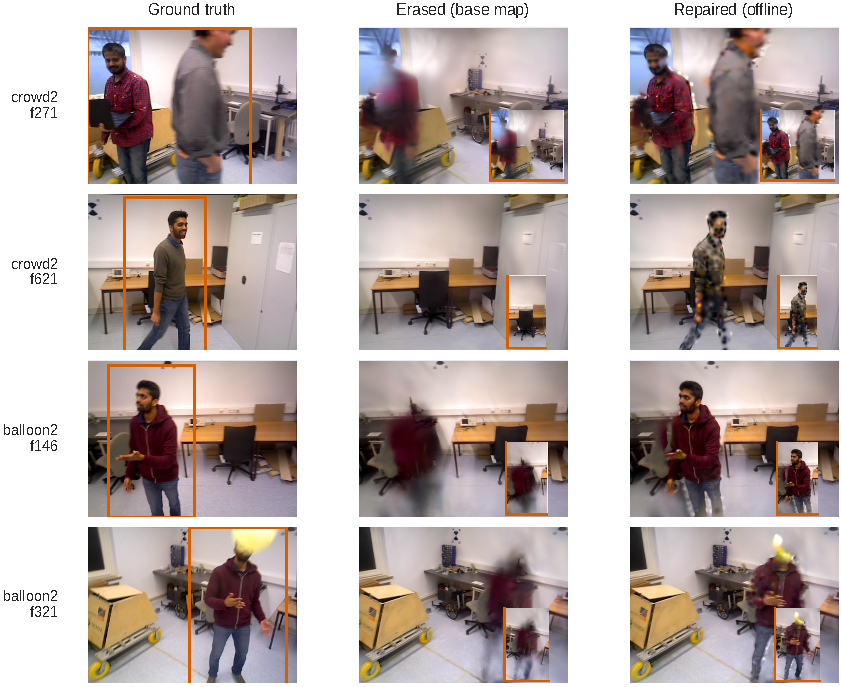
\includegraphics[width=0.70\linewidth]{fig6_dynport_repair.pdf}
\caption{Offline repair on two sequences (crowd2, balloon2), two frames each,
rendered at the evaluated frame's own pose. Columns are ground truth, the base map with dynamic
content erased, and the base map with the dynamic layer restored. The erased people
return without touching the static map; individual inserted primitives are visible at
close zoom, a boundary of this repair path.}
\label{fig:dynport-repair}
\end{figure*}

\section{Discussion and Conclusion}
\label{sec:discussion}

\paragraph{What this paper is and is not.}
This paper studies a map, not a tracker. The system that produces the maps is prior
work, reproduced and reported in \S\ref{sec:system} only to place the map study in a
coordinate frame; its measurements are background, not a claim.
Within that scope, the four map-side questions have concrete answers. The maps of the
system studied here are 30\% constant schema, two exploitable redundancies, and a
load-bearing heavy tail (\S\ref{sec:accounting}). A plain offline codec exploits these
to reach near-lossless $6\times$ compression and $15\times$ at an aggressive working
point, with the gains traced to quantisation and verified on a held-out panel
(\S\ref{sec:codec}). The anti-dynamic policy that produces the map pays a measurable
content cost, recoverable in large part by geometry alone (\S\ref{sec:dyncost}). And an
offline repair operator puts the erased content back as a layer sequence, passing
\gate{21/21} cells across seven sequences and three seeds (\S\ref{sec:offline}). % gate2: manifest_offline_L1_L3.json (21 cells)

\paragraph{Scope conditions.}
Four scope conditions delimit the claims of this study. First, the offline measurements use frozen maps and an offline renderer; they
quantify what the map holds and what an offline operator can recover, not what an
online system achieves; an online placement of the same mechanism shows higher cost
under the snapshot instrument. Second, the repair output is a layer sequence, not a
drop-in replacement for the merged map; the codec quantises both forms, but the
layered form is consumed by its own temporal mechanisms and serves a different
consumer than the merged PLY. Third, the evidence base is two indoor benchmarks
(BONN dynamic, TUM); the held-out panel is drawn from the same two, so the readings
are out-of-sequence but not out-of-benchmark. Within that base, cost and repair come from
one prior stack's maps; the anatomy adds a second system's, a cross-system check on the
anatomy only. The codec's working points generalise to the held-out panel; the other
readings establish what holds for these maps, not a cross-system law. Fourth, the absolute
map sizes here are a few megabytes, so the honest unit of comparison is the ratio and bytes
per primitive.

\paragraph{Limitations and future work.}
This study works within several constraints that future work can address. The
evidence is RGB-D only; monocular splatting SLAM systems exist and one was reproduced
in \S\ref{sec:system}, but the repair operator requires depth to unproject geometry,
and the ground-truth-depth oracle of \S\ref{sec:dyncost} uses ground-truth depth, so the
offline measurements are RGB-D throughout. The repair quality depends on the mask
pathway inherited from the prior stack; better masks would tighten the dynamic-region
bounds, and mask failures propagate directly into misplaced geometry. The layer
sequence is not a drop-in replacement for applications that consume the merged PLY
form; adoption would require a renderer or downstream tool that handles temporal
layers, though the codec already compresses both forms. The anatomy, cost and repair
readings come from one prior stack's maps; a second system's maps enter only the descriptive
anatomy comparison of \S\ref{sec:accounting}. Cross-system generalization of the cost and
repair measurements would require reproducing them on other systems' maps, and whether the
same recovery rates hold across architectures is an open question. Finally, an online system
that manages dynamic content without erasing it remains unbuilt; the offline repair bounds
what such a system could recover, but building an online form that maintains the static
region while keeping dynamic content would require solving the per-frame overhead and
coupling problems that make the online placement unaffordable here.

\paragraph{Why the map deserves attention.}
The map is what a dynamic-scene SLAM system stores, ships and reloads, and the object every
downstream consumer touches. It does not look like what a generic compressor would assume, yet
a deliberately plain codec compresses it well, and the anti-dynamic policy's cost is
concentrated and recoverable. The repair operator points one step further: dynamic content can
be managed outside the online loop, with the static map untouched.

\paragraph{Conclusion.}
We study the maps produced by a dynamic-scene RGB-D splatting SLAM system on their own terms.
We open one, find the schema dead weight and the load-bearing tail, compress it to a sixth of
its size at no visible loss with a parameter-free codec, quantify what the anti-dynamic policy
erases and how much geometry alone recovers, and restore the erased content offline across the
full sequence-and-seed grid. The map of a dynamic-scene SLAM system is worth treating as a
first-class object, and both its compression and its repair admit simple offline answers.

\paragraph{Availability.}
Code, map PLYs, tracking outputs, the codec, and the rendering and evaluation scripts are
released at publication; every number is generated from logged artifacts by those scripts
rather than copied by hand. During anonymous review the artifacts are available from the
authors on request, and the anonymous version of the prior-work paper~\cite{RoGSSLAM} is
included with the supplementary material.

%%%%%%%%% REFERENCES
\bibliographystyle{cvm}
\bibliography{cvmbib}

\end{document}
